% !TeX root = ../main.tex
\documentclass[./../main.tex]{subfiles}

\begin{document}

\subsection{Mô hình ca sử dụng}

\subsubsection{Sơ đồ chính}

Hình \ref{fig:use_case_diagram} mô tả tác nhân và ca sử dụng chính của hệ thống.

\begin{figure}[h!]
	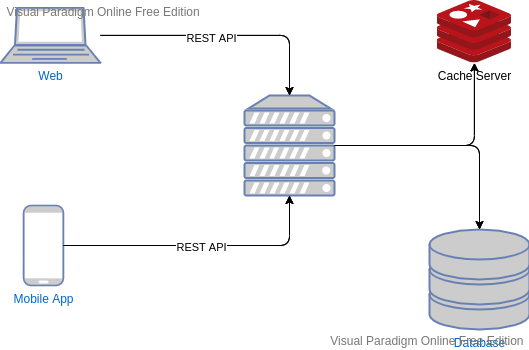
\includegraphics[width=\linewidth]{./images/image4.png}
	\caption{Mô hình ca sử dụng}
	\label{fig:use_case_diagram}
\end{figure}

\subsubsection{Tác nhân của hệ thống}

\begin{itemize}
	\item

	      \textbf{Người dùng} là người đã có tài khoản để truy cập vào hệ thống.

	\item

	      \textbf{Sinh viên} là người dùng hệ thống, sử dụng hệ thống để đăng ký
	      thực tập, nộp báo cáo và xem kết quả thực tập.

	\item

	      \textbf{Giảng viên} là người dùng hệ thống, sử dụng hệ thống để quản
	      lý và chấm điểm cho danh sách sinh viên đang hướng dẫn.

	\item

	      \textbf{Đối tác} là người dùng hệ thống, sử dụng hệ thống để quản lý
	      bài đăng tuyển dụng, danh sách yêu cầu thực tập và danh sách sinh viên
	      đang thực tập tại đơn vị.

	\item

	      \textbf{Quản trị viên Khoa} là người dùng hệ thống, sử dụng hệ thống
	      để quản lý danh sách các kỳ thực tập, danh sách sinh viên, đơn vị thực
	      tập, giảng viên theo từng kỳ và thông tin cá nhân của các đối tượng
	      đó.

	\item

	      \textbf{Quản trị viên} là người dùng hệ thống, sử dụng hệ thống để
	      quản lý danh sách các Khoa, danh sách lớp và quản lý tài khoản người
	      dùng hệ thống.

\end{itemize}

\subsection{Yêu cầu chức năng}

\hypertarget{quux1ea3n-luxfd-buxe0i-ux111ux103ng-cux1ee7a-muxecnh}{%
	\subsubsection{Quản lý bài đăng của
		mình}\label{quux1ea3n-luxfd-buxe0i-ux111ux103ng-cux1ee7a-muxecnh}}

Người dùng \textbf{đối tác} có thể:

\begin{itemize}
	\item

	      Xem, tìm kiếm bài đăng

	\item

	      Chỉnh sửa và tạo mới bài đăng để tuyển dụng thực tập sinh.

\end{itemize}

\hypertarget{quux1ea3n-luxfd-yuxeau-cux1ea7u-thux1ef1c-tux1eadp-cux1ee7a-sinh-viuxean}{%
	\subsubsection{Quản lý yêu cầu thực tập của sinh
		viên}\label{quux1ea3n-luxfd-yuxeau-cux1ea7u-thux1ef1c-tux1eadp-cux1ee7a-sinh-viuxean}}

Người dùng \textbf{đối tác} có thể:

\begin{itemize}
	\item

	      Xem, lọc, tìm kiếm sinh viên

	\item

	      Chấp nhận yêu cầu sinh viên

	\item

	      Từ chối yêu cầu của sinh viên

\end{itemize}

\hypertarget{quux1ea3n-luxfd-sinh-viuxean-ux111ang-thux1ef1c-tux1eadp-tux1ea1i-cuxf4ng-ty}{%
	\subsubsection{Quản lý sinh viên đang thực tập tại công
		ty}\label{quux1ea3n-luxfd-sinh-viuxean-ux111ang-thux1ef1c-tux1eadp-tux1ea1i-cuxf4ng-ty}}

Người dùng \textbf{đối tác} có thể xem, lọc, tìm kiếm sinh viên.

\hypertarget{quux1ea3n-luxfd-kux1ef3-thux1ef1c-tux1eadp}{%
	\subsubsection{Quản lý kỳ thực
		tập}\label{quux1ea3n-luxfd-kux1ef3-thux1ef1c-tux1eadp}}

Người dùng \textbf{quản trị viên Khoa} có thể tạo kỳ thực tập mới. Một
kỳ thực tập bao gồm những thông tin sau:


\textbf{Danh sách công ty cho phép đăng ký thực tập} Người dùng sinh
viên chỉ có thể đăng ký thực tập với các công ty nằm trong danh sách
này. Khi tạo, danh sách các công ty đối tác còn hiệu lực của khoa này sẽ
được tự động thêm vào danh sách cho phép đăng ký của kỳ thực tập. Ngoài
ra, quản trị viên cũng có thể thêm hoặc xóa bỏ công ty trong danh sách
cho phép một cách thủ công.

\textbf{Thời hạn thực tập} Khoảng thời gian 2-3 tháng mà trong đó sinh
viên được phép đăng ký thực tập.


Khi tạo 1 kỳ thực tập mới, cho phép tạo luôn danh sách các công ty đối
tác được chấp nhận trong kỳ này bằng 2 cách: chọn các công ty đã có
trong CSDL và bổ sung các công ty mới. Sau khi có danh sách này, các bài
đăng sẽ \textbf{tự động được sinh ra} (nội dung trống) để cho sinh viên
đăng ký. Sau khi có danh sách này, hệ thống sẽ tự động hiển thị form
đăng ký cho tất cả công ty trong kỳ thực tập.

\hypertarget{quux1ea3n-luxfd-danh-suxe1ch-sinh-viuxean-ux111ang-thux1ef1c-tux1eadp}{%
	\subsubsection{Quản lý danh sách sinh viên đang thực
		tập}\label{quux1ea3n-luxfd-danh-suxe1ch-sinh-viuxean-ux111ang-thux1ef1c-tux1eadp}}

Người dùng \textbf{quản trị viên Khoa} có thể:

\begin{itemize}
	\item

	      Xem danh sách sinh viên đang thực tập

	\item

	      Lọc, tìm kiếm và sắp xếp danh sách sinh viên thực tập

	\item

	      Tải danh sách sinh viên sau khi lọc

	\item

	      Gửi thông báo trúng tuyển hoặc thông báo trượt phỏng vấn

\end{itemize}

\hypertarget{quux1ea3n-luxfd-danh-suxe1ch-ux111ux1ed1i-tuxe1c-trong-kux1ef3-thux1ef1c-tux1eadp}{%
	\subsubsection{Quản lý danh sách đối tác trong kỳ thực
		tập}\label{quux1ea3n-luxfd-danh-suxe1ch-ux111ux1ed1i-tuxe1c-trong-kux1ef3-thux1ef1c-tux1eadp}}

Người dùng \textbf{quản trị viên Khoa} có thể:

\begin{itemize}
	\item

	      Xem danh sách đối tác trong kỳ thực tập

	\item

	      Lọc, tìm kiếm và sắp xếp danh sách đối tác

	\item

	      Chấp nhận/từ chối công ty trong kỳ thực tập

\end{itemize}

\hypertarget{quux1ea3n-luxfd-buxe0i-ux111ux103ng-cux1ee7a-tux1ea5t-cux1ea3-ux111ux1ed1i-tuxe1c-trong-kux1ef3-thux1ef1c-tux1eadp}{%
	\subsubsection{Quản lý bài đăng của tất cả đối tác trong kỳ thực
		tập}\label{quux1ea3n-luxfd-buxe0i-ux111ux103ng-cux1ee7a-tux1ea5t-cux1ea3-ux111ux1ed1i-tuxe1c-trong-kux1ef3-thux1ef1c-tux1eadp}}

Người dùng \textbf{quản trị viên khoa} có thể:

\begin{itemize}
	\item

	      Xem, tìm kiếm bài đăng

	\item

	      Tạo và chỉnh sửa tất cả bài đăng trong khoa của mình.

	\item

	      Ngoài ra, có thể xét duyệt bài đăng của đối tác. Chỉ những bài đăng
	      được duyệt mới được hiển thị cho sinh viên.

\end{itemize}

\hypertarget{quux1ea3n-luxfd-giux1ea3ng-viuxean-hux1b0ux1edbng-dux1eabn-trong-kux1ef3-thux1ef1c-tux1eadp}{%
	\subsubsection{Quản lý giảng viên hướng dẫn trong kỳ thực
		tập}\label{quux1ea3n-luxfd-giux1ea3ng-viuxean-hux1b0ux1edbng-dux1eabn-trong-kux1ef3-thux1ef1c-tux1eadp}}

Người dùng \textbf{quản trị viên khoa} có thể thêm / sửa giảng viên
hướng dẫn cho sinh viên. Sau khi thêm xong, người này có thể gửi danh
sách sinh viên hướng dẫn tới mail của từng giảng viên.

\hypertarget{quux1ea3n-luxfd-danh-suxe1ch-sinh-viuxean}{%
	\subsubsection{Quản lý danh sách sinh
		viên}\label{quux1ea3n-luxfd-danh-suxe1ch-sinh-viuxean}}

Người dùng \textbf{quản trị viên Khoa} có thể xem, lọc, tìm kiếm thông
tin cá nhân của sinh viên trong Khoa.

\hypertarget{quux1ea3n-luxfd-danh-suxe1ch-ux111ux1ed1i-tuxe1c}{%
	\subsubsection{Quản lý danh sách đối
		tác}\label{quux1ea3n-luxfd-danh-suxe1ch-ux111ux1ed1i-tuxe1c}}

Người dùng \textbf{quản trị viên Khoa} có thể:

\begin{itemize}
	\item

	      Xem, tìm kiếm, lọc danh sách công ty liên kết và công ty ngoài trong
	      Khoa

	\item

	      Thêm và sửa liên hệ cho công ty

\end{itemize}

\hypertarget{quux1ea3n-luxfd-danh-suxe1ch-giux1ea3ng-viuxean}{%
	\subsubsection{Quản lý danh sách giảng
		viên}\label{quux1ea3n-luxfd-danh-suxe1ch-giux1ea3ng-viuxean}}

Người dùng \textbf{quản trị viên Khoa} có thể xem, tìm kiếm danh sách
người dùng giảng viên trong Khoa.

\hypertarget{quux1ea3n-luxfd-ngux1b0ux1eddi-duxf9ng}{%
	\subsubsection{Quản lý người
		dùng}\label{quux1ea3n-luxfd-ngux1b0ux1eddi-duxf9ng}}

Người dùng \textbf{quản trị viên} có thể thêm / sửa thông tin người dùng
trên hệ thống. Thông tin người dùng bao gồm:

\begin{itemize}
	\item

	      Thông tin cá nhân: tên, email, ngày sinh, mã số sinh viên, \ldots{}

	\item

	      Thông tin đăng nhập: tên đăng nhập, mật khẩu, ...

\end{itemize}

\hypertarget{quux1ea3n-luxfd-danh-suxe1ch-khoa}{%
	\subsubsection{Quản lý danh sách
		khoa}\label{quux1ea3n-luxfd-danh-suxe1ch-khoa}}

Người dùng \textbf{quản trị viên} có thể thêm / sửa / xóa Khoa và quản
lý tài khoản quản trị viên cho Khoa đó.

\hypertarget{quux1ea3n-luxfd-danh-suxe1ch-lux1edbp}{%
	\subsubsection{Quản lý danh sách
		lớp}\label{quux1ea3n-luxfd-danh-suxe1ch-lux1edbp}}

Người dùng \textbf{quản trị viên} có thể thêm / sửa /xóa lớp.

\hypertarget{cac-yeu-cau-chuc-nang-khac}{%
	\subsubsection{Các yêu cầu chức năng khác}\label{cac-yeu-cau-chuc-nang-khac}}

Ngoài các yêu cầu chức năng nêu trên, còn có các yêu cầu chức năng khác của hệ thống được trình bày ở khóa luận của bạn Lại Tuấn Anh:

\begin{itemize}
	\item

	      Đăng nhập hệ thống

	\item

	      Đặt lại mật khẩu

	\item

	      Đổi mật khẩu

	\item

	      Chỉnh sửa thông tin cá nhân

	\item

	      Xem thông tin bài đăng

	\item

	      Đăng ký thực tập với công ty liên kết

	\item

	      Đăng ký thực tập với công ty ngoài

	\item

	      Đăng ký phỏng vấn từ bài đăng

	\item

	      Xem thông tin thực tập

	\item

	      Chọn công ty để thực tập

	\item

	      Nộp báo cáo thực tập

	\item

	      Tải lên CV

	\item

	      Xem thống kê dữ liệu trên hệ thống

	\item

	      Xem danh sách sinh viên đang hướng dẫn

	\item

	      Xem báo cáo thực tập của sinh viên

	\item

	      Chấm điểm cho sinh viên

\end{itemize}

\subsection{Yêu cầu phi chức năng}

Giao diện sản phẩm cần phải thoả mãn yêu cầu về khả năng truy cập. Ngoài
ra, giao diện cần hỗ trợ nhiều kích cỡ màn hình khác nhau và tuân thủ
theo nguyên tắc thiết kế của trường Đại Học Quốc Gia Hà Nội.

\end{document}